\documentclass{article}

% if you need to pass options to natbib, use, e.g.:
%     \PassOptionsToPackage{numbers, compress}{natbib}
% before loading neurips_2021

% ready for submission
\usepackage[preprint, nonatbib]{neurips_2021}

% to compile a preprint version, e.g., for submission to arXiv, add add the
% [preprint] option:
%     \usepackage[preprint]{neurips_2021}

% to compile a camera-ready version, add the [final] option, e.g.:
%     \usepackage[final]{neurips_2021}

% to avoid loading the natbib package, add option nonatbib:
%    \usepackage[nonatbib]{neurips_2021}

\usepackage[utf8]{inputenc} % allow utf-8 input
\usepackage[T1]{fontenc}    % use 8-bit T1 fonts
\usepackage[colorlinks=true]{hyperref}       % hyperlinks
\usepackage{url}            % simple URL typesetting
\usepackage{booktabs}       % professional-quality tables
\usepackage{amsfonts}       % blackboard math symbols
\usepackage{nicefrac}       % compact symbols for 1/2, etc.
\usepackage{microtype}      % microtypography
\usepackage{xcolor}         % colors
\usepackage{multirow}
\usepackage{graphicx}
\usepackage{caption}
\usepackage{subcaption}
\usepackage{wrapfig}
\usepackage{float}
\usepackage[sorting=none]{biblatex} %Imports biblatex package
\addbibresource{bibliography.bib} %Import the bibliography file

\title{Automatic book genre classification}

\author{%
  Vera Milovanović\\
  University of Tübingen\\
  \texttt{vera.milovanovic@student.uni-tuebingen.de}
  \And
  Yeong Hwangbo\\
  University of Tübingen\\
  \texttt{yeong.hwangbo@student.uni-tuebingen.de}
  \And
  Filip Radović\\
  University of Tübingen\\
  \texttt{filip.radovic@student.uni-tuebingen.de}\\
}


\begin{document}


\maketitle


\begin{abstract}
  We use the collection of \href{https://www.cs.cmu.edu/~dbamman/booksummaries.html}{books} to see whether we could classify them into the predefined set of genres using only the book summaries.  For this purpose, we are planning to use complement naive Bayes, logistic regression, random forest, and XGBoost and compare their performances. The project repository on GitHub can be found \href{https://github.com/radovic/automatic-book-genre-classification}{here}.
\end{abstract}


\section{Introduction}

In recent times, especially after the start of the Covid-19 pandemic, the proportion of books sold online has drastically increased. Often, people's search criteria are genres, which could also help online bookstores to identify one’s preferences. Therefore, a book recommendation system that uses genre classification would be useful for customers as well as for online bookstores to increase their profit. \\ \\
In this project, we perform the analysis on CMU Book Summary Dataset that contains plot summaries for 16,559 books extracted from Wikipedia, along with aligned metadata from Freebase, including publication dates, authors, book titles, and book genres. We classify the collection of books into the predefined set of genres using the book summaries. For this purpose, we apply TF-IDF vectorization of summaries and additional data pre-processing. We conduct label filtering to reduce the set of genres to the most commonly known. Then we implement four models for multi-label classification and compare their performances using different types of metrics. 


\section{Experiments}

\subsection{Data pre-processing}

For the first dataset used in this project, out of 277 labels, i.e. genres from the original dataset, some are dropped as they represent a tag rather than genre, for example, \textit{morality play} and \textit{sea story}. Others are grouped around the broader genres, for example, \textit{cyberpunk}, \textit{military science fiction}, \textit{time travel} are grouped as \textit{science fiction}. In this way, we largely denoise our dataset, as there are lots of infrequent genres that mostly do not represent commonly known genres. Figure 1 shows the final 15 genres used for the classification and their frequency. \\
\begin{wrapfigure}{r}{0.4\textwidth}
\centering
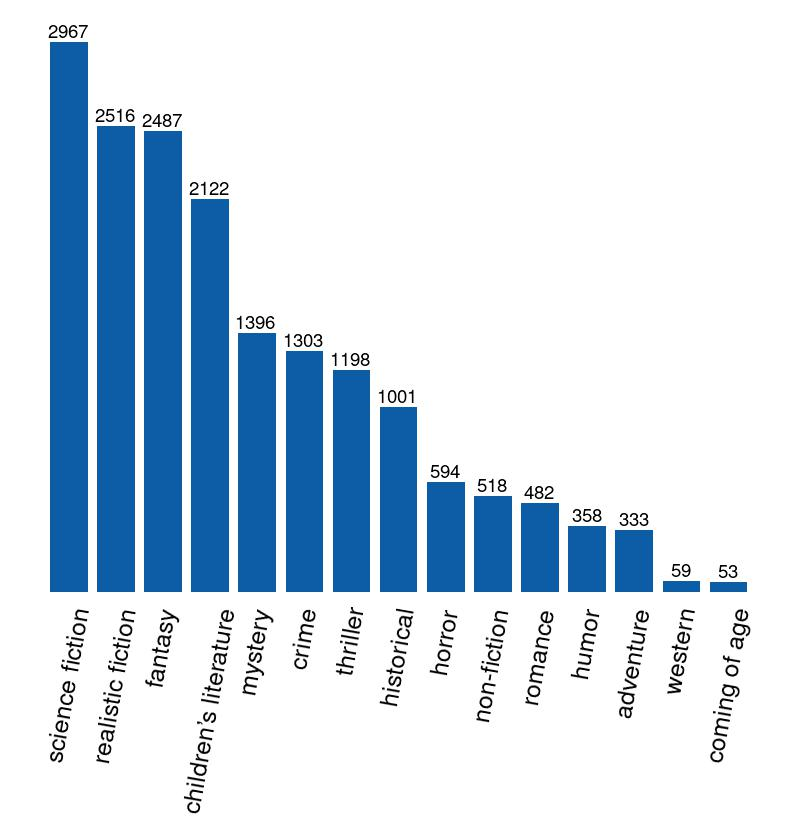
\includegraphics[width=\linewidth]{../../gfx/genrecounts.jpg}
\caption{\small{Number of books per genre}}
\label{fig:figure1}
\end{wrapfigure} 
In order to possibly improve the performances of the classification we drop genres from the previously mentioned dataset with the lowest F1 scores obtained after classification. The genres with the F1 score below the 0.4 threshold are dropped, leaving 9 labels for the second dataset. \\
We transform summaries from the filtered datasets into the vectors using TF-IDF vectorization \cite{ramos2003using}. TF-IDF is an algorithm that assigns weights to terms depending on how relevant they are to the corpus on which it is performed. Inspired by Zipf's law \cite{newman2005power}, before the vectorization apply some additional steps. First, we tokenize the corpus and remove all tokens that are either stop words or contain non-alphabetic characters as we want to have only informative features. The remaining words are lemmatized, i.e. reduced to their dictionary form, in order to avoid having different weights for different inflected forms of the same word. \\
We also exclude words with small frequencies in the datasets because we want to reduce the vocabulary and avoid potential overfitting caused by the connection of the terms which are scarcely represented in the training set to specific genres. It is done by iterative search of the cut-off value on the interval $[0, 0.001]$. It represents the minimal portion of texts that should contain each word of the corpus. By comparing the accuracy of the complement Bayes model we come to the optimal cut-off value of $0.125\%$.

\subsection{Classification}

The pipeline for the classification process is the same for both datasets. In order to prevent selection bias and subsequently underestimating the generalization error, hyperparameter tuning is conducted independently from the fitting and evaluation procedures in each trial \cite{cawley2010over}. For this purpose, k-fold nested cross-validation is used, where the inner 2-fold loop serves for hyperparameter tuning and the outer 5-fold loop for generalization error estimation. Additionally, as the first step in the model pipeline, TF-IDF vectorization is applied to test and train folds of the outer loop independently, so data leakage into the test sets is prevented. Random search cross-validation is used for the hyperparameter tuning for all models except for complement Naive Bayes for which hyperparameter tuning is not conducted. For logistic regression inverse of regularization strength is tuned, and for random forest and XGBoost it is the maximum depth of the trees. We tune only one hyperparameter with three search iterations to reduce the number of fittings, which are especially time-consuming with XGBoost. During the process of hyperparameter tuning and generalization error estimation, we keep track of the three evaluation metrics: F1 score(micro), accuracy, and Hamming loss. The best model found during the hyperparameter search is fitted on the train sets using F1 micro score.  \\
We compare the generalization errors of the Complement Naive Bayes \cite{rennie2003tackling}, logistic regression \cite{bishop2006pattern}, random forest \cite{ho1995random} and XGBoost \cite{chen2016xgboost}. We use the Complement Naive Bayes classifier instead of the other versions because it was shown that the Complement Naive Bayes preceded by TF-IDF with normalization performed well \cite{rennie2003tackling}. In the rest of this report, we will call this model transformed weight-normalized Complement Naive Bayes, or TWCNB for short. \\
Since we have a multi-label problem, and TWCNB, logistic regression and XGBoost do not support it, we transform the multi-label classification to the two-class problem using OneVsRestClassifier, i.e. fitting one classifier per class. Random forest inherently supports multi-label classification \cite{breiman2001random}. \\
In order to compare the models’ performances, we choose three metrics: Accuracy, F1 score(micro), and Hamming loss. Micro F1 score and Hamming loss are chosen because they weigh all samples evenly and all classes are equally important to us. Additionally, accuracy is used because it counts labels as incorrectly predicted if they do not entirely match the true set of labels. Contrary to accuracy, Hamming loss acknowledges partially correct classification which is important for multi-label classification. \\

\section{Results}

\begin{table}[ht]
\centering
\begin{tabular}{ |p{2cm}|p{2cm}||p{2cm}|p{2cm}|p{2cm}|  }
 \hline
 Dataset & Model name & F1 score (micro) & Accuracy & Hamming loss\\
 \hline \hline \hline
\multirow{4}{*}{15 genres} & TWCNB & 0.5572 $\pm$ 0.0030 & 0.3158 $\pm$ 0.0033 & 0.0780 $\pm$ 0.0006\\ \cline{2-5}
 & LR & \textit{0.5629} $\pm$ 0.0030 & \textit{0.3305} $\pm$ 0.0018 & \textbf{\textit{0.0709}} $\pm$ 0.0006 \\ \cline{2-5}
 & RF & 0.2361 $\pm$ 0.0121 & 0.1192 $\pm$ 0.0048 & 0.1044 $\pm$ 0.0017 \\ \cline{2-5}
 & XGBoost & 0.5138 $\pm$ 0.0027 & 0.2783 $\pm$ 0.0020 & 0.0774 $\pm$ 0.0005 \\ \hline \hline
\multirow{4}{*}{9 genres} & TWCNB & \textbf{\textit{0.6049}} $\pm$ 0.0023 & 0.3671 $\pm$ 0.0058 & 0.1123 $\pm$ 0.0010 \\ \cline{2-5}
 & LR & 0.6025 $\pm$ 0.0021 & \textbf{\textit{0.3760}} $\pm$ 0.0058 & \textit{0.1035} $\pm$ 0.0010 \\ \cline{2-5}
 & RF & 0.2577 $\pm$ 0.0095 & 0.1291 $\pm$ 0.0056 & 0.1642 $\pm$ 0.0029 \\ \cline{2-5}
 & XGBoost & 0.5602 $\pm$ 0.0030 & 0.3266 $\pm$ 0.0051 & 0.1144 $\pm$ 0.0011 \\ \hline
\end{tabular} \\
\caption{ \small{Mean scores and their standard errors of different models for each dataset \\ The values written in cursive are the best scores obtained from the dataset, and the values written in bold are the best obtained values per metric on both datasets. The higher F1 score and accuracy and the lower Hamming loss the better classification is.}}
\label{tab:table1}
\end{table}

Overall, by comparing the results in Table 1, we note that logistic regression has the best performance on both datasets. We also note that TWCNB and logistic regression have similar performances, so TWCNB might be the preferred model because of its simplicity and training time (Figure 2). It is also worth mentioning that none of the scores has an error greater than 0.01. \\ 
Although we anticipated better results on the dataset with a smaller number of genres, we see only slight improvement in F1 score and accuracy of the models. In the case of Hamming loss, we also see the increase in the value. However, this is not as bad as it seems, since Hamming loss is greatly influenced by the imbalance of the classes. For example, if we take one of the minority classes, coming-of-age (0.5\% of books), the Hamming loss for the classifier that does not assign anything to coming-of-age would be less than 0.005 which is almost perfect result. Therefore, it would drastically pull the overall Hamming loss down and make an illusion of good classification. \\
\begin{figure}[h]
\begin{subfigure}{.5\textwidth}
  \centering
  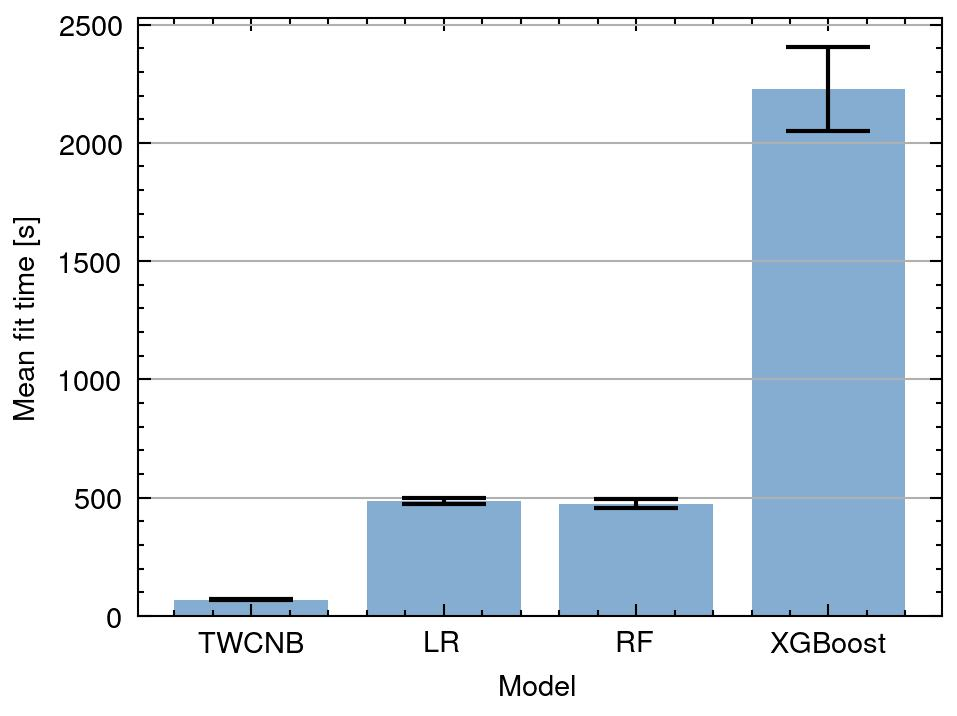
\includegraphics[width=.9\linewidth]{../../gfx/redgenrestimes.jpg}
  \caption{9 genres dataset}
  \label{fig:sub1}
\end{subfigure}%
\begin{subfigure}{.5\textwidth}
  \centering
  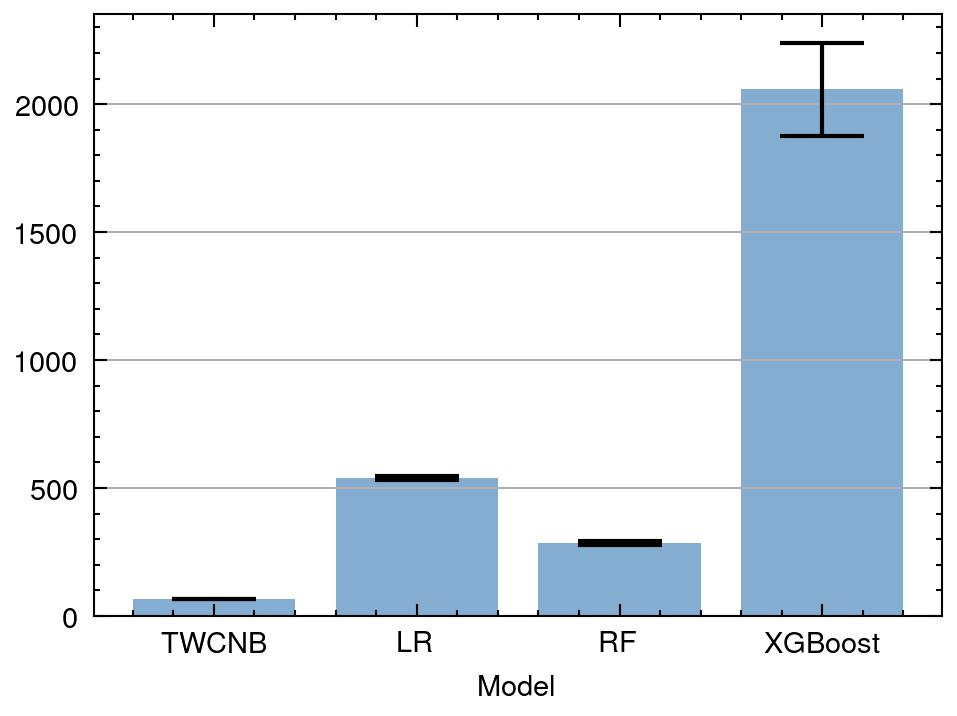
\includegraphics[width=.9\linewidth]{../../gfx/allgenrestimes.jpg}
  \caption{15 genres dataset}
  \label{fig:figure2}
\end{subfigure}
\caption{\small{Mean fit times and their standard deviations}}
\label{fig:test}
\end{figure} \\
In addition, since the standard errors of random forest in Table 1 are notably greater than those of the other models, we conjecture that this model is more sensitive to the hyperparameter change. Not surprisingly, since XGBoost is the most complex model among other models we test here, it takes the longest time to fit the data (Figure 2). Varying the value of XGBoost's hyperparameter maximum depth of trees does not influence the scores (Table 1). However, as we can see by the standard deviation of the mean training time in Figure 2, it significantly influences the training time. Therefore, it is better to keep the max depth at lower values, for example, 2. 

\section{Fairness}
Conducting this kind of classification raises some questions about the fairness of the model. 
According to the \cite{graham2015digital}, Wikipedia is characterized by highly uneven geographies of participation. This result is in compliance with our finding that non-western authors are in minority in the dataset used in this project, as only book articles in English were collected. This possibly makes the classification model biased toward recognizing books in a “western” writing style. \\
Moreover, the dataset contains disproportionally more male authors, which introduces a bias toward assigning certain genres to the book according to the gender of the writer. A study \cite{argamon2003gender} showed that there was a significant difference in male versus female writing style, which confirms our claim.
Both of the previously mentioned fairness concerns should be taken into account if such kinds of models were used in a book recommendation system.

\section{Limitations and future work}
In this section, we suggest some modifications to the proposed classification procedure. \\
Our project has two main limitations. The first is the size and imbalance of the CMU dataset. Even before grouping and filtering the labels, more than 22\% of the dataset is unlabeled and consequently useless for our project. The other problem is that the dataset is imbalanced. For example, the prevalence of the most frequent genre is 55 times greater than the most infrequent one. The second limitation is of technical nature, hyperparameter search was extremely time-consuming so we had to restrict the hyperparameter spaces accordingly. Hence, it might be that the random search used for hyperparameter tuning did not find the optimal hyperparameters for our models. \\
The dataset could be better exploited if other features were used, for example, the book author and the publishing date. However, this would immensely increase the dimensionality of the problem, as each author should be encoded. Also, summaries could be transformed differently, which would result in better performance. We propose Doc2Vec\cite{le2014distributed} or trying different n-gram models. 

\section{Conclusion}
We conclude that the proposed models do not perform well in assigning genres to books. We assume that is because summaries do not contain features that are discriminative enough. However, it should be pointed out that the classifier deals with a big number of possible genres. On the other hand, the results are consistent, as the estimate of the standard error of the means of all metrics is negligible.

\printbibliography

\end{document}